\section{Introduction}
In PET imaging one of the needs in many clinical and research applications is acquisition of information over the whole body. Moreover, dynamic information over the whole body can allow for research applications of PET, such as in pharmacokinetics, to expand to the whole body and enable potential future clinical applications. 
An important limitation of DWB protocols in scanners with limited A-FOV is the result temporal gaps in the acquired data of any given bed position. These are introduced at each bed position by the time spent on imaging other bed positions and from the time required to move the bed to the next position and prepare for the next acquisition. 
In practice for scanners that have no in-build DWB protocols, such as the Signa PET/MR, a large fraction of the acquisition delays in DWB protocols are attributed to a greater extend to system processes that are lunched automatically between WB sweeps rather than to time taken to move the bed between bed positions. These processes include transfer of raw data files and reconstructions performed during scanning. More acquisition time could be gained if those could be avoided and delays were decreased.

In this chapter we review results of acquisition performance from a dynamic whole-body (DWB) protocol implemented on the Signa PET/MR scanner as part of the IsotoPK pharmacokinetic study~\cite{Marie2019}. A short introduction on the design of the protocol using current scanner features is privded here, with details on processing and exportation of the data provided in Appendix~\ref{chap:AppendixA}.
We then describe the implementation of an experimental fully-automated protocol for DWB acquisitions on the Signa PET/MR, that was designed with the aim of reducing acquisition delays and allow for greater flexibility in selection of bed positions. The development of this protocol was conducted as part of this project and in collaboration with GE Healthcare. 
Finally, we present results of the experimental acquisition protocol applied on a \gls{nhp} study and compare against the standard DWB protocol used in the IsotoPK study with data from fourteen volunteer scans.

\section{Methods \& Results}

\subsection{Design of IsotoPK DWB protocol on the Signa PET/MR}
Prior to commencing this PhD project and in perpetration for the IsotoPK study, a DWB protocol was designed on the GE Signa PET/MR scanner. The desired coverage was achieved using 5 bed positions and a reduced overlap, as shown in diagram (C) of figure~\ref{fig3_1:BodyCoverage}. The relatively small overlap (half compared to routine clinical protocols) was selected to reduce the number of beds and subsequently the acquisition temporal gaps.
The study design was limited to a total duration of 1 hour from injection and includes an initial dynamic single bed (DSB) phase centred over the liver, where the highest expression of the transporters under study was expected. 
The DWB position was imaged for 3 minutes from injection, prior to the start of DWB acquisition.
Because the system has no in-build protocols for DWB imaging, a custom protocol had to be made using a series of static WB acquisition protocols. Each WB pass had to be individually pre-planned, which resulted in fixed bed positions (relevant to a reference mark). Each volunteer positioning was made using a chest-landmark, with no further adjustments of the protocol allowed for optimum positioning of the bed positions, relative to each patient's size.

For the design of the framing used in the IsotoPK DWB protocol, the following empirical metric has been taken under consideration. We define the Delays to Acquisition ratio (DAR) as the ratio of total delays to acquisition time for every WB sweep, using the relationship
\begin{equation} \label{eqn:acq_to_dead_time}
 \mathrm{DAR} = \frac{dl_{bed}\cdot 4 + dl_{Sweep}^{(5)}}{t_{duration}\cdot 5 }  \\ , \\ 
\end{equation}
where $t_{duration}$ is the frame duration for a single bed in the WB sweep, $dl_{bed}$ the delays between adjacent beds and $dl_{Sweep}^{(5)}$ the delay between WB sweeps (for a DWB protocol of 5 bed positions).
First estimations of the delay times for the Signa PET/MR had shown a delay of approximately 6 seconds between adjacent bed positions and 20 seconds between WB sweeps. Using this information, the framing sequence shown in table~\ref{tab:IsotoPK_Framing} was chosen with the shortest frame duration set to 20 seconds in order to maintain a DAR lesser than 50\% at the early phases of the DWB study. 

\begin{table}[]
\caption{Framing of IsotoPK DWB protocol.}
\label{tab:IsotoPK_Framing}
\begin{tabular}{|l|l|l|l|l|}
\toprule
\textbf{Phase ID} & \textbf{Description}              & \textbf{Frame Duration (s)} & \textbf{Number of Frames} & \textbf{DAR} \\
\midrule
1        & DSB & 10                 & 18        & N/A                 \\
2        & DWB                      & 20                 & 9         & 44\%                \\
3        & DWB                      & 30                 & 8         & 29\%                \\
4        & DWB                      & 40                 & 2         & 22\%                \\
\bottomrule
\end{tabular}
\end{table}

MR sequences required for attenuation correction (MRACs) were performed prior and during the DWB protocol acquisition. The first MRAC sequence at each bed location lasted approximately 35 seconds, with subsequent scans over the same locations lasting approximately 21 seconds per bed. MRAC acquisitions were not repeated for all WB sweeps of the DWB protocol, to allow for entry in the room for blood sampling which is required for derivation of the input function and metabolite analysis. 
%A details description of the WB sweeps is given in the appendix. %(refereed in protocol naming as \textit{CE}, standing for whole body "corps entier" in French)

The acquired DWB data were initially reconstructed at the system console.
Then, as part of this PhD project, the raw data were retrospectively exported for offline processing and treated with the steps of an automated pipe-line described in Appendix~\ref{chap:AppendixA}.

\subsection{Results from IsotoPK study}

The result beds positions of the DWB protocol can be seen in figures~\ref{fig3_1:ctrl_mips} and ~\ref{fig3_1:rif_mips} for the fourteen studies of the IsotoPK protocol evaluated.
Using the timing information of the extracted raw PET data, the average delay times per imaged subject were estimated, shown in the form of box-plots for $dl_{bed}$ in figure~\ref{fig3_1:BoxPlots_beds} and for $dl_{Sweep}^{(5)}$ in figure~\ref{fig3_1:BoxPlots_sweeps}.

It is noteworthy that with accumulation of experience in using the PET/MR system for performing the DWB protocol the delays between sweeps were reduced considerably, which can be seen by comparing the most recent examinations against the first. This can be attributed to improved preparation of the PET/MR system before performing the protocol (ex. reboot of the system prior to acquisition, etc.).
For the 3 more recent subject examinations the average intra-bed delay time $dl_{bed}$ was 5.69 s (95\%CI: 5.63,5.75) and the average delay time between sweeps $dl_{Sweep}^{(5)}$ was 26.17 s (95\%CI: 26.13, 26.22).
The average $dl_{Sweep}^{(5)}$ value was slightly higher than the value considered in the design of the protocol. With those average measurements the DAR for the WB sweeps with the shortest frame duration is approximately 49\%. \\

%
\begin{figure} [ht!]
\centering
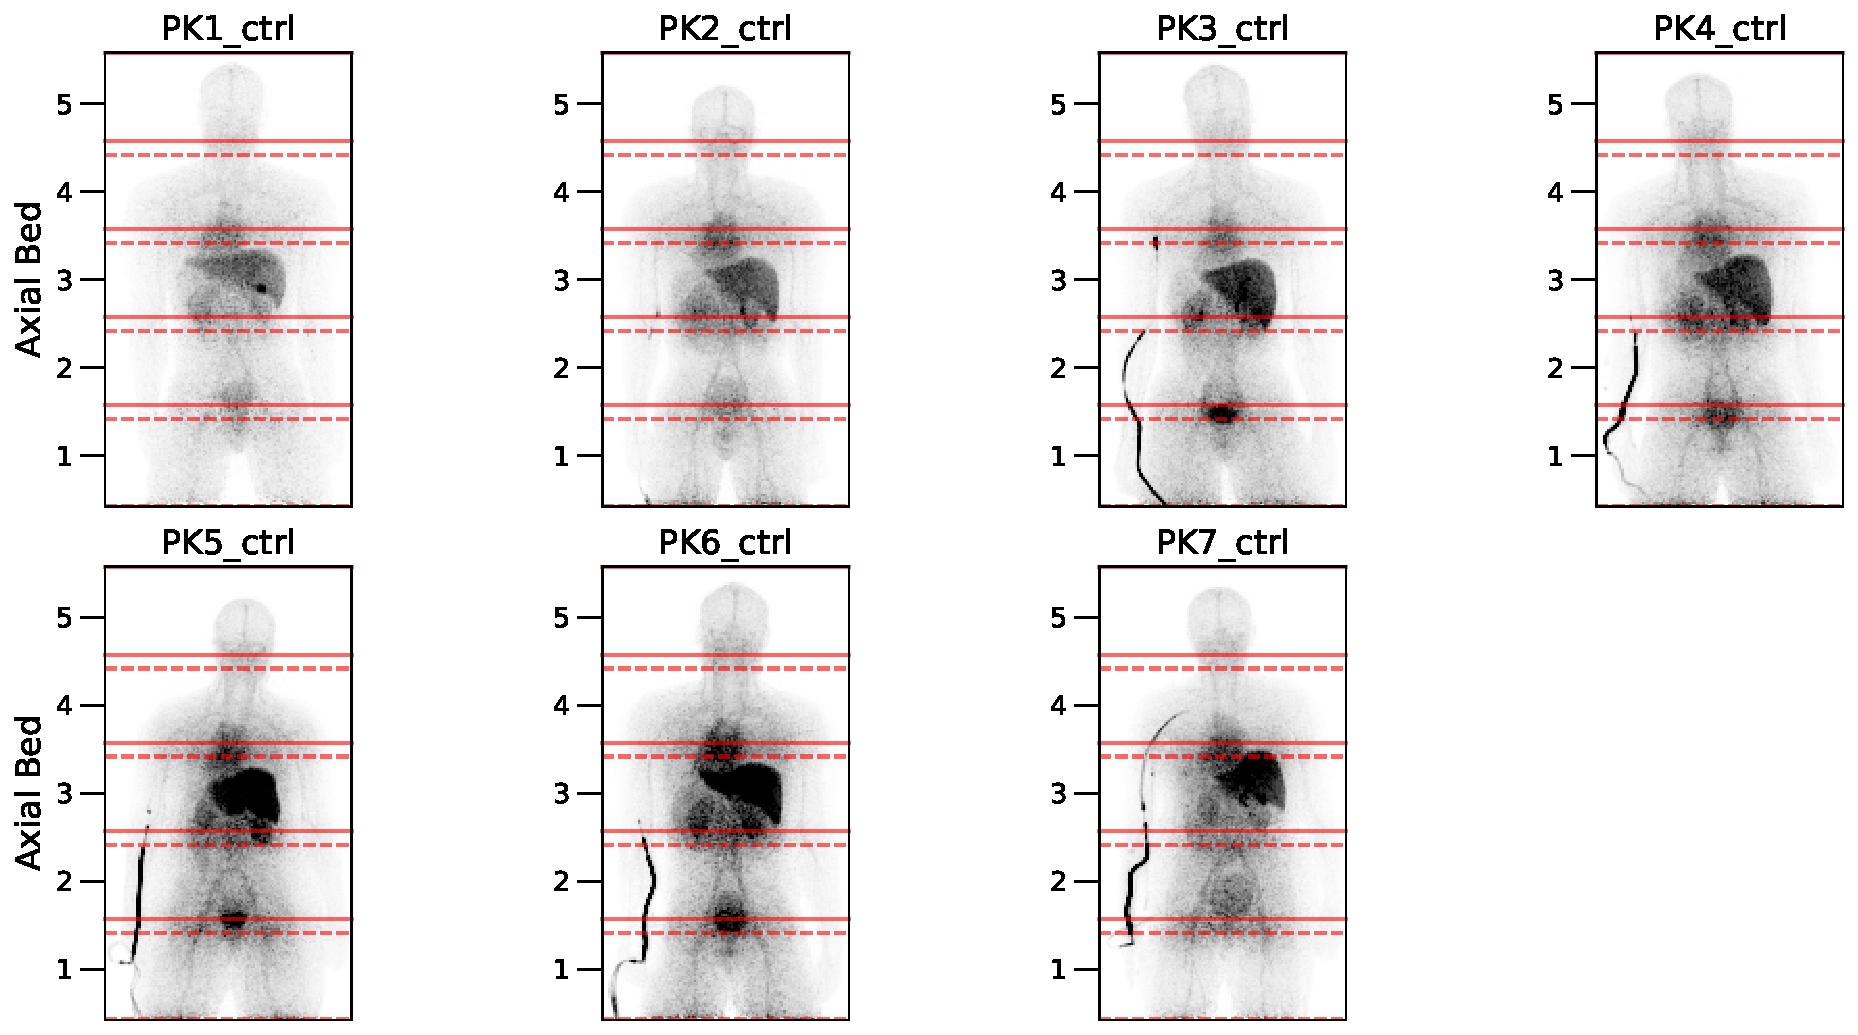
\includegraphics[scale=0.5,angle=0]{3_Results/3_1_DWB_Optimization/figures/3_1_MIPS_ctrl.pdf}
\caption{MIP projections of 7 volunteer control DWB scans with overlay of axial bed start and end location.} 
%TODO: Add over-scan in the CBM D-WB protocols. 
\label{fig3_1:ctrl_mips}
\end{figure}
%
\begin{figure} [ht!]
\centering
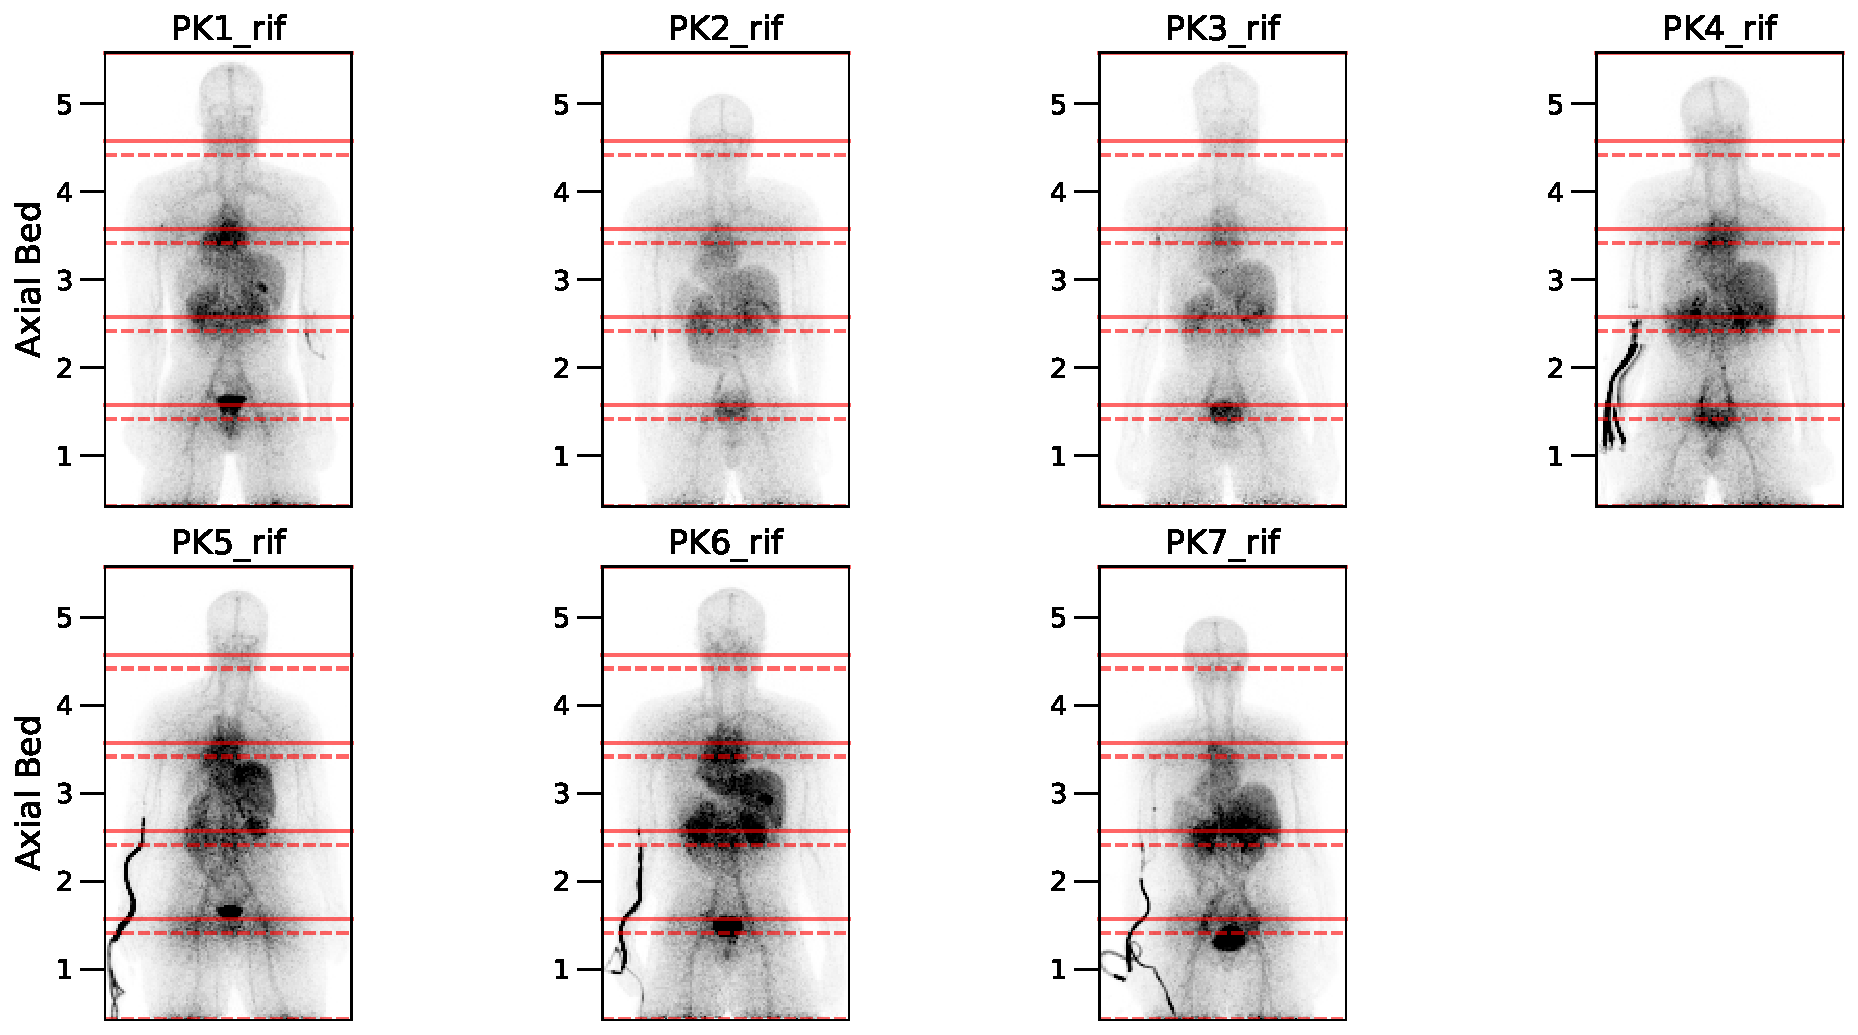
\includegraphics[scale=0.5,angle=0]{3_Results/3_1_DWB_Optimization/figures/3_1_MIPS_rif.pdf}
\caption{MIP projections of 7 volunteer rif DWB scans with overlay of axial bed start and end location.} 
%TODO: Add over-scan in the CBM DWB protocols. 
\label{fig3_1:rif_mips}
\end{figure}
%
%
%
\begin{figure} [ht!]
\centering
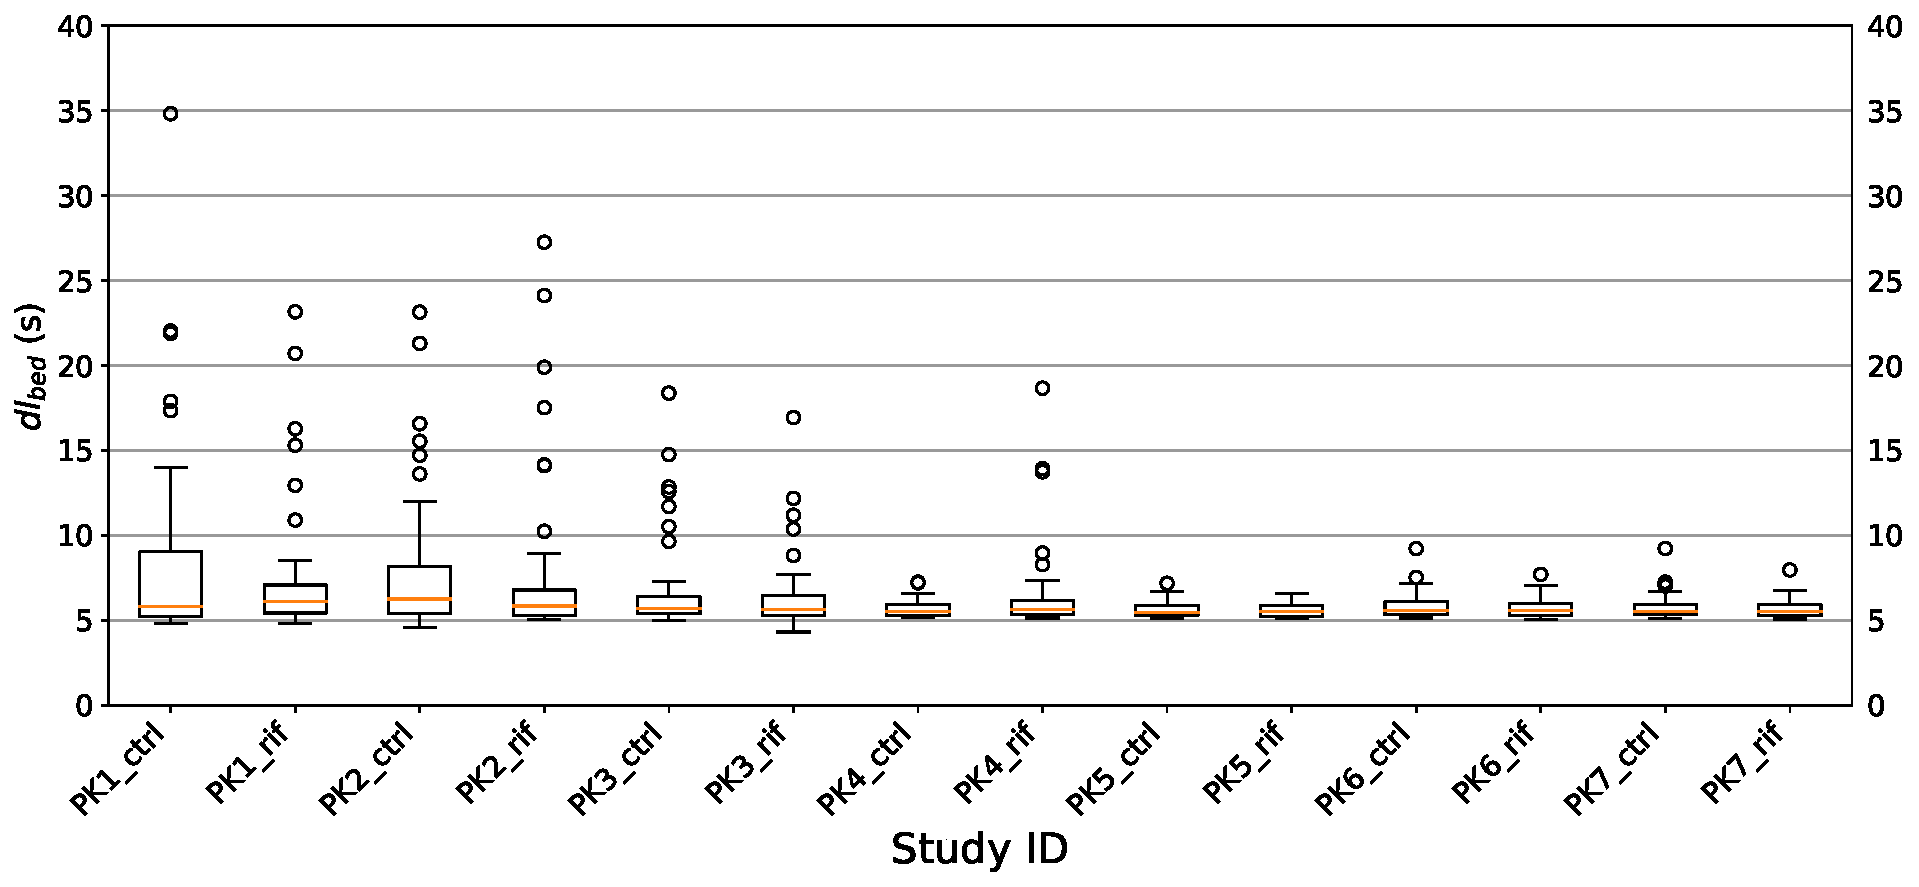
\includegraphics[scale=0.5,angle=0]{3_Results/3_1_DWB_Optimization/figures/3_1_BoxPlots_DTBeds.pdf}
\caption{Box plots of intra-bed delays $dl_{bed}$ of the IsotoPK DWB protocol used in practice.} 
%TODO: Add over-scan in the CBM D-WB protocols. 
\label{fig3_1:BoxPlots_beds}
\end{figure}
%
\begin{figure} [ht!]
\centering
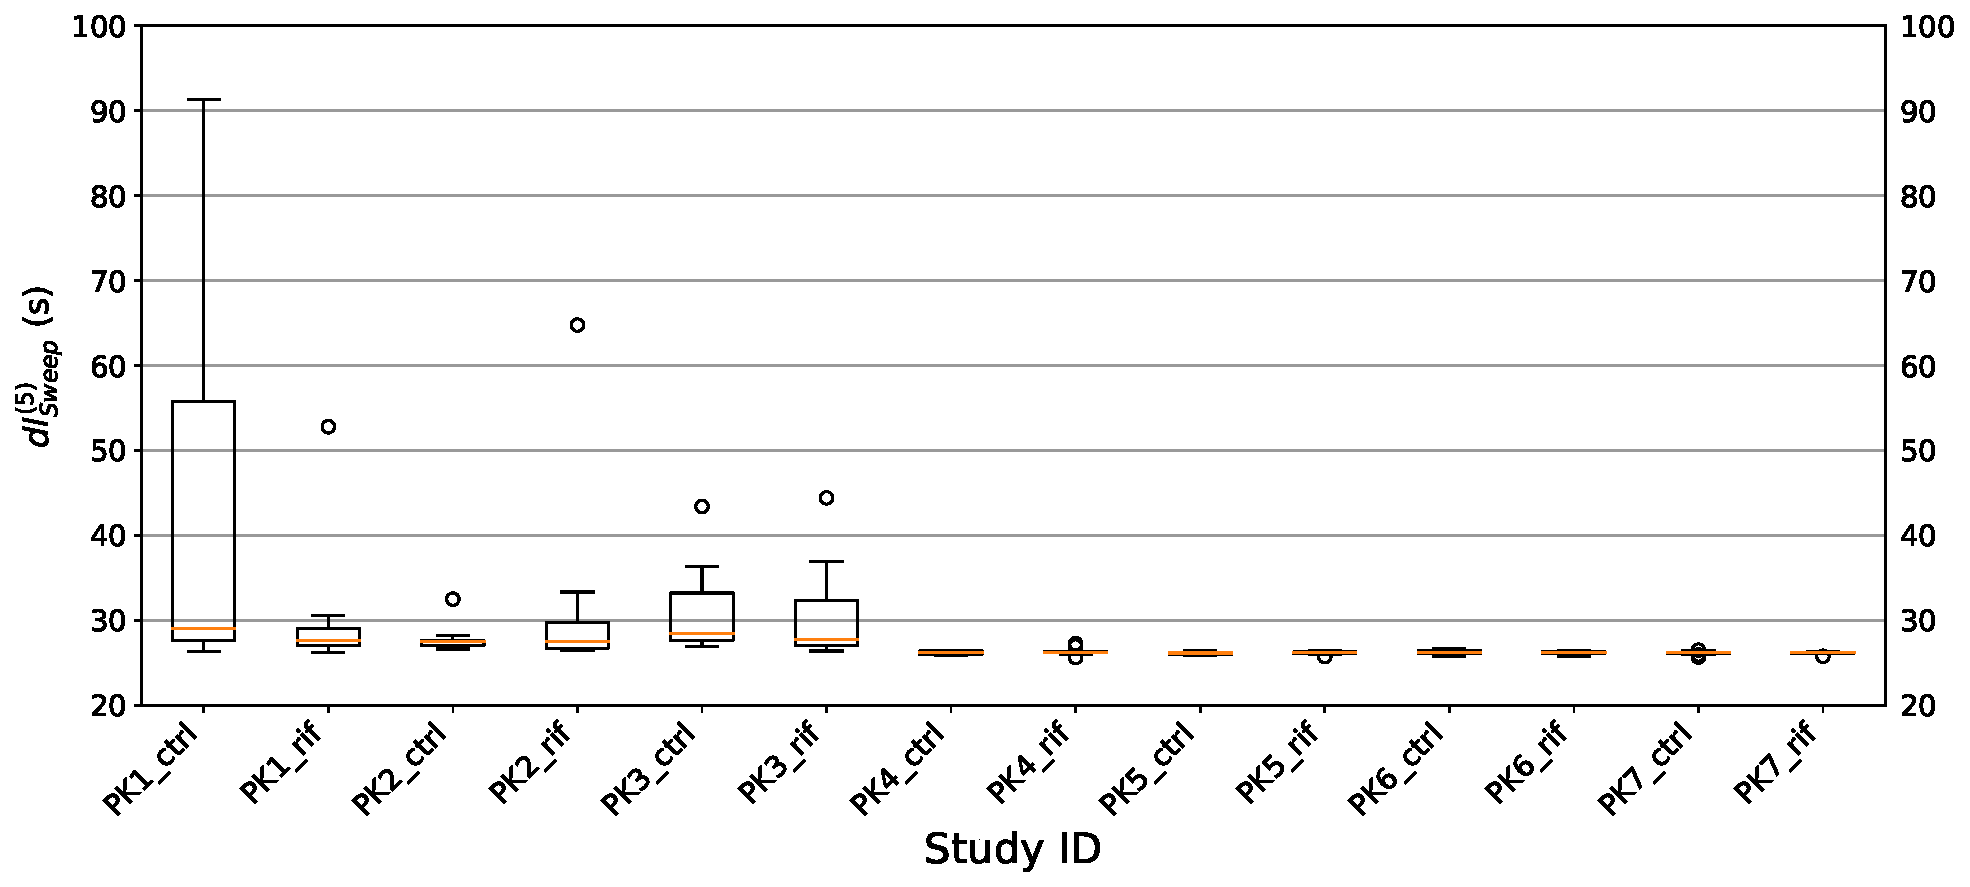
\includegraphics[scale=0.5,angle=0]{3_Results/3_1_DWB_Optimization/figures/3_1_BoxPlots_DTSweeps.pdf}
\caption{Box plots of delay between WB Sweeps $dl_{Sweep}$ of the IsotoPK DWB protocol used in practice.}
%TODO: Add over-scan in the CBM D-WB protocols. 
\label{fig3_1:BoxPlots_sweeps}
\end{figure}
%
%
%
\subsection{Design of a fully-automated DWB protocol on the Signa PET/MR}
Part of this PhD project was allocated for the development of a fully-automated DWB protocol on the Signa PET/MR. 
The main requirement for the envisioned protocol was to allow for continuous capture of PET data during DWB acquisition, into a single list-mode file for all bed positions. Then the data could be processed after acquisition, split to individual data for each bed position and reconstructed with the correct bed positional information. Using such an acquisition strategy the delays between bed positions and WB sweeps could be reduced to the time taken by the physical motion of the scanner table alone. 

Towards this goal, the PhD project schedule included a four week industrial secondment with GE healthcare, for the purpose of exploring tools that could enable the automation of DWB protocols. Three weeks of this secondment were spend at factory facilities of GE healthcare (Waukesha, Wisconsin, USA). %with the opportunity the gain insights on the operations of the Signa PET-MR scanner. 
There with help of the PET/MR team it was made possible to exploit in-build factory tools of the Signa PET/MR for the purposes of DWB automation. The two key tools necessary were: 
\begin{itemize}
    \item\textbf{Table Emulation} \\
    This tool allows for disassociation of the table position between the MR and PET system. It is the key tool that allows for the PET system to acquire continuously, while the MR system governs table motion. The disadvantage of this functionality is that once table emulation is enabled MR acquisitions cannot be performed.% while acquiring PET data.
    \item\textbf{Table Motion} \\
    This tool commands the MR system to execute movements of the scanner bed. It can be used to drive the bed to a target location at a desired speed. 
\end{itemize}

The automated DWB protocol was implemented as a Python class, because the python programming language is available on the PET/MR system's console and allowed for easy integration of the system tools with our custom made routines, all under a common system clock for accurate timing of bed movements and registration of events.
The protocol was named "Auto-IsotoPK", but despite its name is a generic DWB protocol that is not limited to the IsotoPK pharmacokinetic study. It allows for an optional DSB scan to be acquired before starting the DWB acquisition. It also allows for any number of beds to be used for DWB acquisition, with custom positioning of the beds for each examination using an initial MR scout image. 
Because MR acquisitions cannot be performed after \textit{Table Emulation} is enabled, all bed position MRACs must be acquired prior to the PET examination and used for all WB sweeps of the study.

A short \gls{sop} on the operation of the protocol is given in Appendix~\ref{chap:AppendixA}.

After the procedure is completed, the whole PET study is stored as a single list-mode file. The precise timing information of the acquired bed positions are saved in a log file, to be used for the post-processing procedure prior to reconstruction.  

\subsection{Results from NHP study}
After initial tests using phantoms, the automated DWB protocol was tested on an actual pre-clinical DWB study. A macaque was scanned under full sedation with a novel $^{18}$F-Crizotinib tracer, that was being investigated for uses in \gls{nsclc} disease. The DWB study was required to examine tracer uptake in the brain as well as uptake and excretion from other organs. The macaque was injected with 185 \si{\mega \becquerel} of the novel tracer. Directly after injection an initial DSB scan was conducted, centred over the brain for a duration of 90 s, followed by DWB acquisition of 3 bed positions. The study was planned for an approximate total duration of one hour. A total of 28 WB sweeps were fitted in the study, with the framing of 3$\times$10~\si{\s}, 5$\times$20~\si{\s}, 5$\times$30~\si{\s}, 5$\times$45~\si{\s}, 10$\times$60~\si{\s} for each of the three bed positions.

Acquisition of the required MRACs was performed prior to injection, at the planned bed positions shown in figure~\ref{fig3_1:Macaque_MRI}. In this acquisition only the body coils of the PET-MR system were used, which are optimised for use with the human body size, which resulted in sub-optimal quality of MR images and subsequently attenuation maps. The generated attenuation maps required manual editing before used for PET data reconstruction.

\begin{figure} [ht!]
\centering
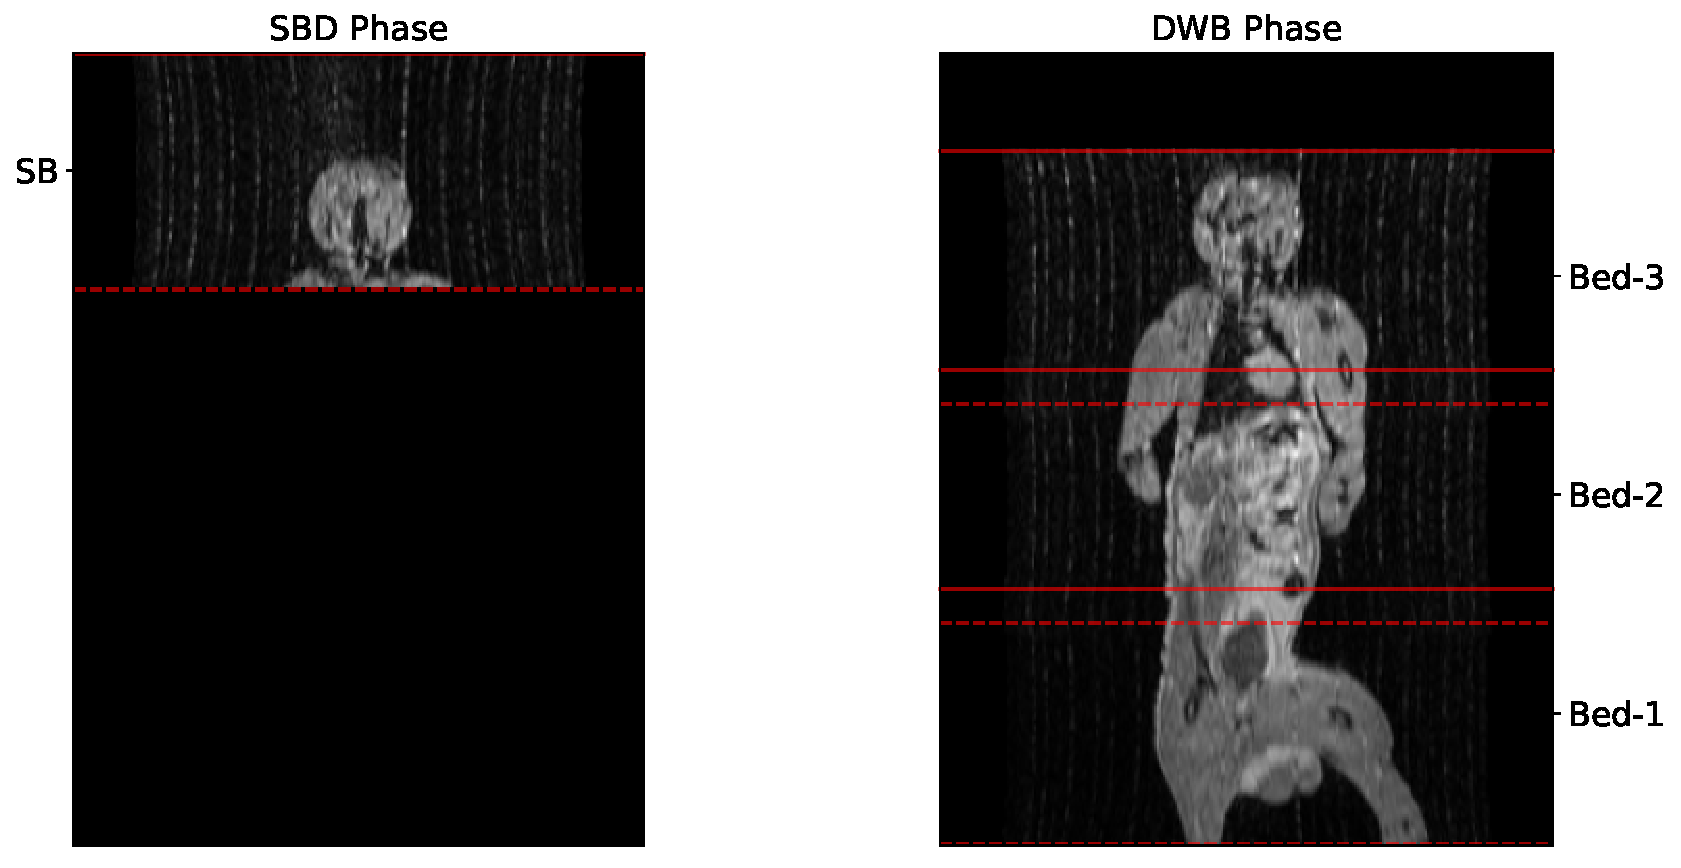
\includegraphics[scale=0.5,angle=0]{3_Results/3_1_DWB_Optimization/figures/3_1_Macaque_MRI.pdf}
\caption{MRAC acquisitions of NHP study showing the planned bed positions of the two acquisition phases.}
\label{fig3_1:Macaque_MRI}
\end{figure}

The complete study dataset was recorded in a single list-mode file, of which the head curve (curve of prompts rate with time) can be seen in figure~\ref{fig3_1:Macaque_Head_Curve}. By overlaying the recorded timing information over this curve, the two phases of the acquisition (DSB and DWB) as well as the three bed position of the DWB acquisition can be distinguished. The initial 260 second of the recorded list-data's head curve with the overlaid phases and bed positions are shown in figure~\ref{fig3_1:Macaque_Head_Curve_Phases}. 

\begin{figure} [ht!]
\centering
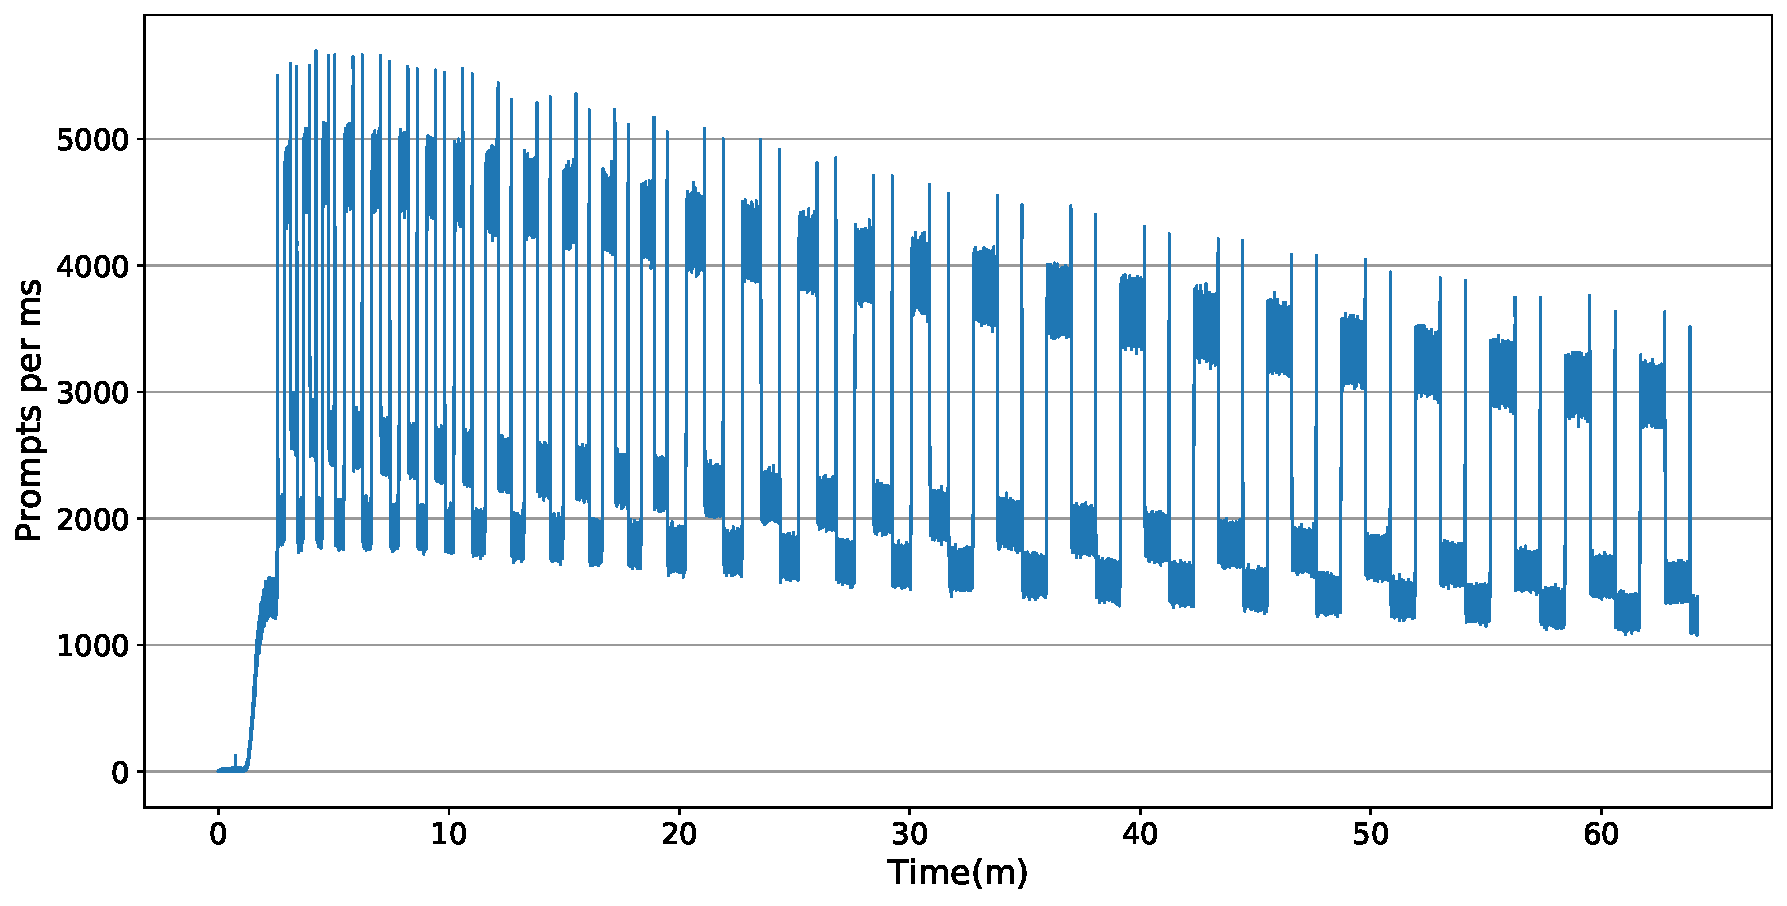
\includegraphics[scale=0.45,angle=0]{3_Results/3_1_DWB_Optimization/figures/3_1_Macaque_Head_Curve.pdf}
\caption{Head curve (prompts rate against time) of the acquired NHP study DWB data in a single list-mode file using the optimised protocol.}
\label{fig3_1:Macaque_Head_Curve}
\end{figure}

\begin{figure} [ht!]
\centering
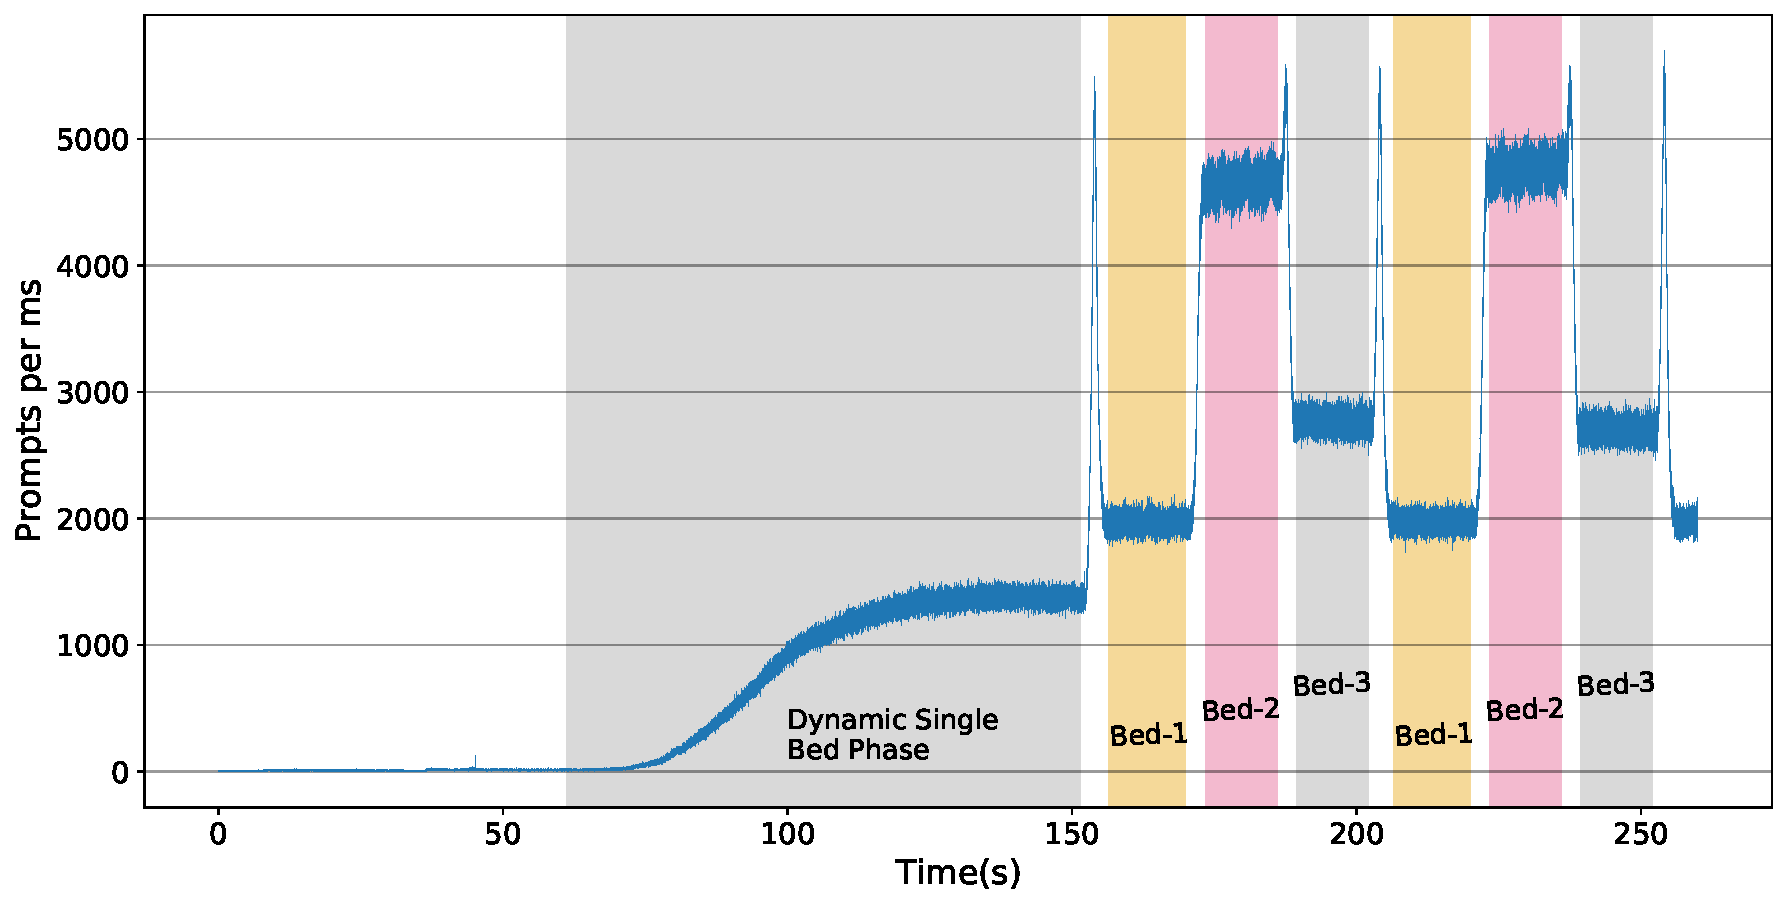
\includegraphics[scale=0.45,angle=0]{3_Results/3_1_DWB_Optimization/figures/3_1_Macaque_Head_curve_Phases.pdf}
\caption{Head curve (prompts rate against time) of the acquired NHP study showing the DSB and DWB phases of the acquisition and the three DWB bed positions.}
\label{fig3_1:Macaque_Head_Curve_Phases}
\end{figure}
%
Using the timing information recorded by in the log file, the data were split into four individual bed position datasets and were processed with the GE-PET toolbox individually as single bed dynamic studies. The list-mode data along with the generated corrections were then exported into the CASToR data-file format for subsequent reconstruction tests. A \gls{mip} view of 3D reconstructions (averaged across all dynamic frames) is shown in figure~\ref{fig3_1:Macaque_PET}. \\
An IDIF was estimated from the PET data, needed for subsequent kinetic analysis of the data. An right carotid VOI was used, which was visible on both phases of the acquisition, and a left ventricle VOI. Both VOIs provided similar blood activity values for the DWB phase and were averaged to produce the final IDIF, shown in figure~\ref{Macaque_PET_input_function}.
%
\begin{figure} [ht!]
\centering
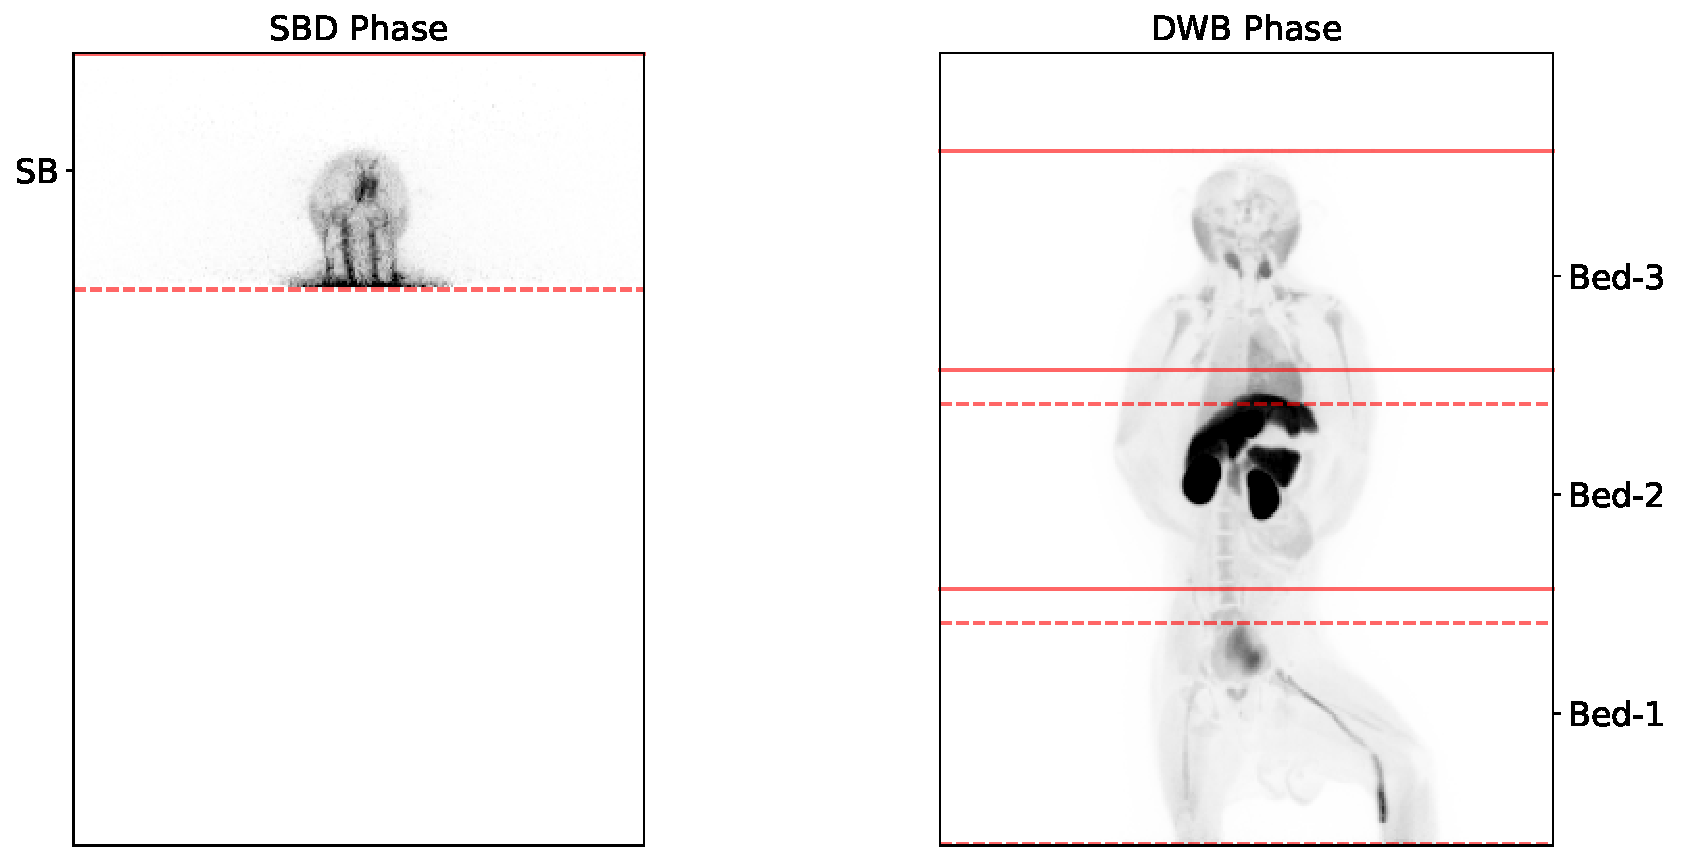
\includegraphics[scale=0.45,angle=0]{3_Results/3_1_DWB_Optimization/figures/3_1_Macaque_PET.pdf}
\caption{MIP views of the NHP study's reconstructed PET images, for the two phases of the acquisition.}
\label{fig3_1:Macaque_PET}
\end{figure}
%
%
\begin{figure} [ht!]
\centering
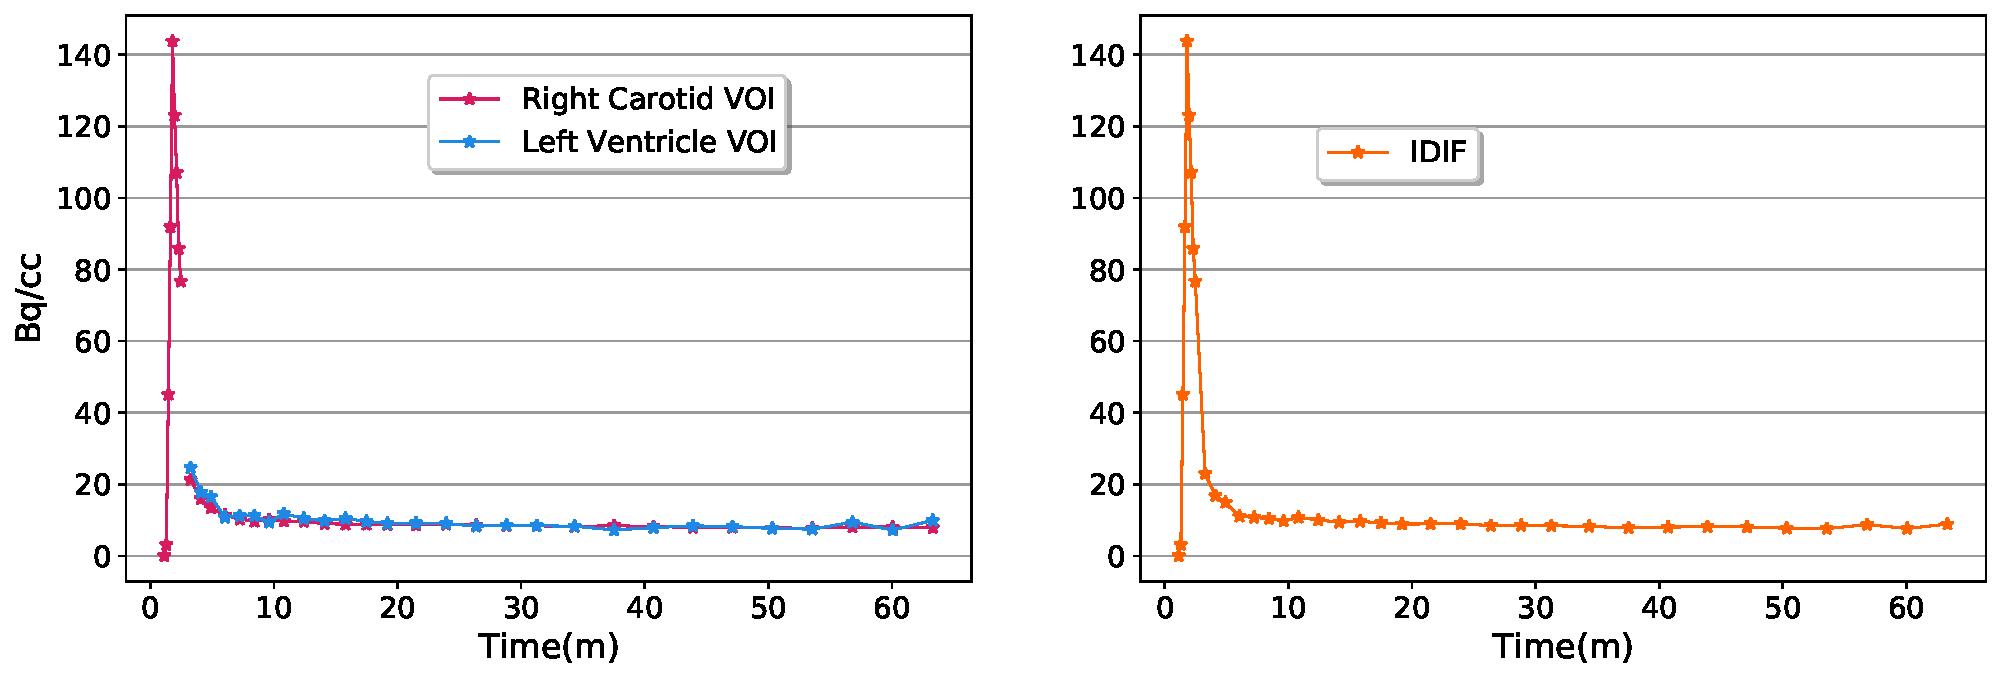
\includegraphics[scale=0.45,angle=0]{3_Results/3_1_DWB_Optimization/figures/3_1_NHP_InputFunction.pdf}
\caption{NHP study's image derived input function using information from multiple bed positions.}
\label{fig3_1:Macaque_PET_input_function}
\end{figure}
%
Finally an estimation of the delays (time gaps) for this single NHP study using the automated acquisition protocol was made using log timing information. The results showed an average intra-bed delay time $dl_{bed}$ of 3.77 s (95\%CI: 3.62,3.91) and an average delay time between sweeps $dl_{Sweep}^{(3)}$ of 4.6 s (95\%CI: 4.53, 4.67). 

\section{Comparison of protocols}
The design and implementation of the fully-automated DWB protocol was made with the intentions of reducing delay times, compared to the custom implementation of a DWB protocol on the Signa PET/MR. 
Before direct comparison of the protocols, the delay times between WB sweeps need to be adjusted to account for the difference in number of bed positions between the tests of the two protocols. 
Assuming a linear relationship between delays due to bed motion and the number of beds, the following relationship can be expressed

\begin{equation} \label{eqn:acq_to_dead_time_ratio}
dl_{{Sweep}}^{(5)} =\ \frac{5}{3} dl_{{Sweep}}^{(3)}  \\ , \\ 
\end{equation}

where now $dl_{Sweep}^{(5)}$ is the delay between sweeps that would be achieved by the fully automated protocol for DWB imaging of 5 bed positions. 
Using the measurements from the NHP study, the $dl_{Sweep}^{(5)}$ achievable is estimated to be 7.66 s. 
Using this value we can estimate that the DAR for 20 s frames can be reduced from 49\% to approximately 22.7\%, by use of the fully automated protocol instead of the current IsotoPK DWB protocol. Furthermore, using the reduced $dl_{Sweep}^{(5)}$ delays a DAR of approximately 45.5\% can be achieved for 10 s frames, allowing for more frequent sampling in the early phases of DWB acquisition without significantly compromising on the quantity of acquisition statistics. 

Additionally, besides the reduced acquisition gaps the fully automated protocol allows for more flexibility in position of bed positions for DWB imaging. By contrast the hard-set bed positions of the IsotoPK DWB protocol do not always allow for optimum use of the effective A-FOV in each examination, as seen for example in examination PK2 in figures~\ref{fig3_1:ctrl_mips}~and~\ref{fig3_1:rif_mips}. In some cases a fewer number of bed positions might be adequate and preferable as it would lead to substantial increase of sampling frequency per bed.

\section{Discussion}

As seen by the reduction of $dl_{Sweep}$ delay time and reduction of DAR for short frame duration, the implementation of the fully-automated DWB protocol resulted in considerable reduction of acquisition delays which leads to reduction of acquisition gaps in DWB data. This gain can be used towards improving statistics of PET raw data of early frames, or towards higher acquisition frequency of early frames for the same level of statistics. 
In the comparisons of the two protocols we used the empirical metric of DAR, without relating that to effects of delays in final kinetic analysis performed on the data and produced parametric images. In general faster sampling can be achieved even with high system delays, at the cost of reduced acquisition statistics and vice versa with higher statistics achieved at the cost of reduced sampling frequency. 
These trade-offs are expected to affect mostly kinetic estimations that rely mostly on early dynamic information shortly after injection. 
Ideally the DWB acquisition protocol should be optimised for the expected kinetics under study. Towards this optimisation, the automated DWB can allow for greater variability in the available options for this trade-off of statistics vs. sampling frequency of early frames. 

Another aspect where fast sampling can be beneficial is for the derivation of the IDIF from DWB data. Given the fast initial sampling that can be achieved using a fully-automated protocol it is possible to reduce the initial DSB acquisition time or remove it completely from 

In this evaluation a limitation that has not been considered is limits on table movement that are needed to avoid effects from electromagnetic induction on patients/volunteers by the fast movement of the bed within the MR field. For the tests conducted on the NHP, these limits have not been considered. These limits are expected to reduce the speed that would be permissive for human subjects, in compliance also with patient comfort requirements, and thus reduce the potential gains from use of the fully automated DWB protocol. 

Finally in our tests we have considered only the use of S\&S acquisition in the implementation and optimisation of DWB protocols. 
In a previous study on DWB protocols utilising CBM acquisition, advantages favouring the use CBM acquisition for DWB protocols were seen~\cite{Karakatsanis2016}. beyond the aspects of reduced acquisition delays, CBM offers other benefits such as uniform axial sensitivity of acquisition, flexibility in sampling frequency by adjustments in table speed within each WB sweep,improved patient comfort, etc. 
Overall use of CBM naturally overcomes many of the limitations posed by use of multi-bed DWB protocols with use of S\&S acquisition. 
Finally, CBM protocols can also allow for bi-directional motion that eliminates delays between WB sweeps. 
These acquisition modes, their effects on acquisition gaps and result parametric image quality were considered further in the simulation study presented in chapter XX.

\section{Conclusion}
A fully automated DWB protocol was developed. Data using this protocol were successfully acquired, processed and reconstructed in a test NHP study.
Use of the protocol allowed for considerable reduction of delay times, enabling faster sampling without loss of PET data statistics.
A considerable limitation of the implementation of this protocol is the unavailability of the MR system for MRI acquisitions during the DWB acquisition, which is caused by the bespoke utilities on which our experimental protocol was based upon.
Finally, further considerations of permissible table speeds for patient safety and comfort need to be applied before using this protocol on human subjects.


%At this moment CBM protocols are not available on the PET/MR scanner, but DWB protocols based on CBM acquisition can overcome many of the limitations and enable even more flexibility in acquisition frequency, with the additional benefits of uniform axial sampling. 

%\subsection{Auto-IsotoPK: Continuous Bed Motion on the Signa PET-MR}
%The flexibility offered by the use of the automated protocol and the dedicated \"Table Motion\" tool allowed for testing the proof of concept of CBM on the Signa PET-MR scanner. Although this acquisition mode is not supported by the system, we emulated the acquisition of a single whole-body sweep by commanding a table movement at a speed of \SI{5}{\milli\metre\per\second}. The duration of the total sweep, that covered the three bed positions that were acquired in the previous DWB study and included an 50\% overscan, was ...